\documentclass[11pt]{article}


\setlength{\parindent}{0pt}
\usepackage{xltxtra}
\usepackage{hyperref}
\hypersetup{hidelinks}
\usepackage{url}
\urlstyle{tt}
\usepackage{xcolor}
\definecolor{CVBlue}{RGB}{23,110,191}
\usepackage{calc}
\usepackage{graphicx}
\usepackage{tikz}
\usetikzlibrary{calc}
\usepackage{fontspec}
\usepackage{xeCJK}
\usepackage{enumitem}
\CJKsetecglue{} %% 取消中文与数字之间的间隙


%%  主文档字体设置
\setmainfont[
    Path = fonts/Main/,
    Extension = .otf,
    BoldFont = texgyretermes-bold.otf, % 加粗字体
]{texgyretermes-regular.otf} % 正文字体

% 中文字体设置
\setCJKmainfont[
    Path = fonts/hansans/,
    Extension = .ttf,
    BoldFont = NotoSansSC-Bold.ttf, % 加粗字体
]{NotoSansSC-Regular.otf} % 正文字体


\usepackage{relsize}
\usepackage{xspace}

% 使用 fontawesome（部分图标）
\usepackage{fontawesome} 

% A4纸， 上下左右边距
\usepackage[
    a4paper,
    left=1.2cm,
    right=1.2cm,
    top=1.5cm,
    bottom=1cm,
    nohead
]{geometry}

\renewcommand{\baselinestretch}{1.5} % 行间距设为1.5

\usepackage{titlesec}
\usepackage{enumitem}
\setlist{noitemsep} % 取消列表项间的额外间距
%\setlist{nosep} % 取消所有垂直间距
\setlist[itemize]{topsep=0.25em, leftmargin=*}
\setlist[enumerate]{topsep=0.25em, leftmargin=*}

% --- 用于控制【不同项目之间】的垂直距离 ---
\newlength{\interProjectSpacing}
\setlength{\interProjectSpacing}{0.9em} % <--- 在此调整项目之间的距离
\newcommand{\projectsep}{\vspace{\interProjectSpacing}}

% --- 用于控制【项目标题】与下方【项目描述】的距离 ---
\newlength{\intraProjectTitleSep}
\setlength{\intraProjectTitleSep}{0.4em} % <--- 在此调整标题和描述的距离
\newcommand{\titlebreak}{\\[\intraProjectTitleSep]}

% --- 用于控制【项目描述】与下方【要点列表】的距离 ---
\newlength{\intraProjectListTopSep}
\setlength{\intraProjectListTopSep}{0.2em} % <--- 在此调整描述和列表的距离

% =======================================================================


\titleformat{\section}         % 定制 \section 命令 
{\large\bfseries\raggedright} % 将 section 标题设置为大号、粗体且左对齐
{}{0em}                      % 可用于为所有 section 添加前缀（如“章节...”）
{}                           % 可用于在标题前插入代码
[{\color{CVBlue}\titlerule}]  % 在标题后插入一条横线
\titlespacing*{\section}{0cm}{*1.6}{*1.2}



\begin{document}
\pagenumbering{gobble}

%%%% 利用tikz来定位照片
\begin{tikzpicture}[remember picture, overlay] 
    \node[anchor = north east] at ($(current page.north east)+(-2cm,-1.2cm)$) {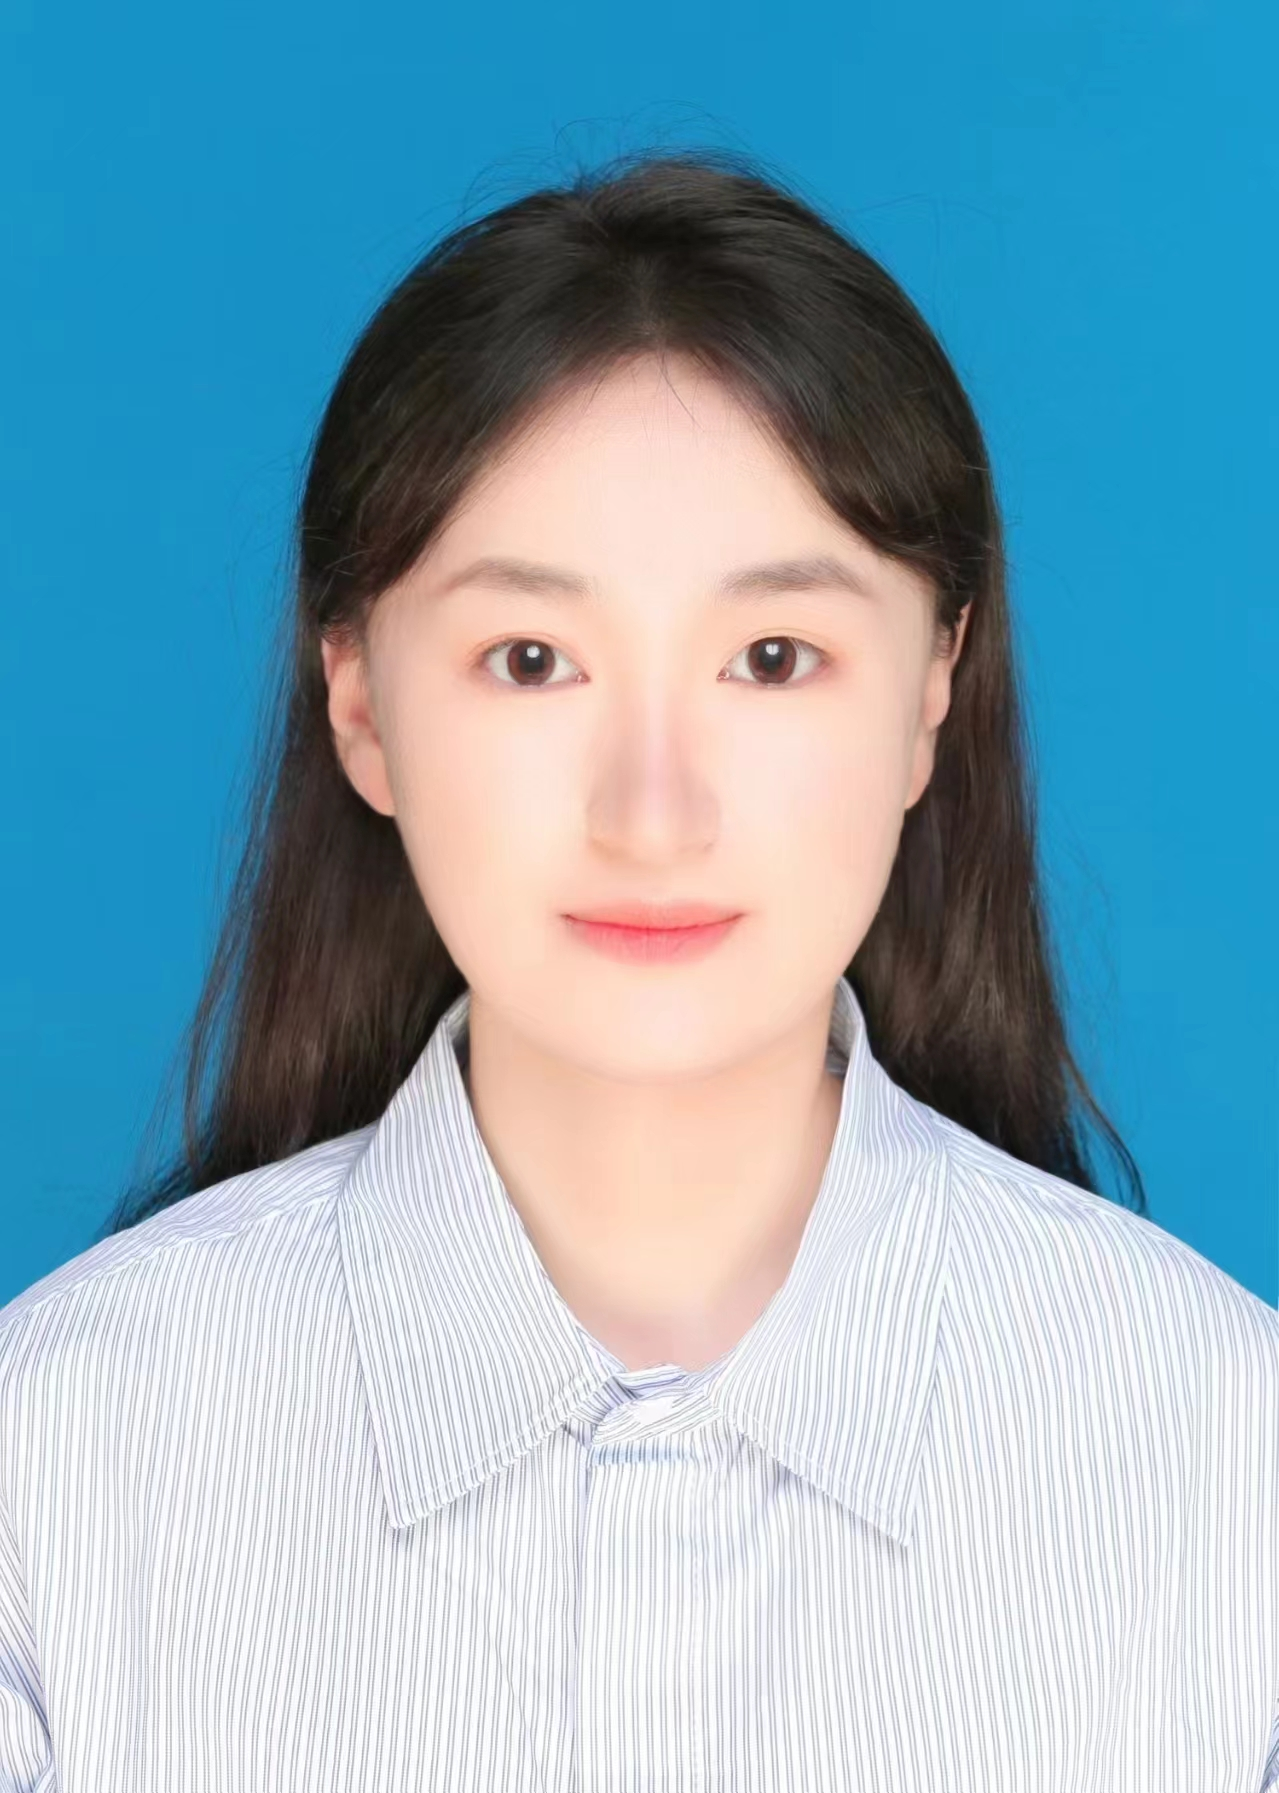
\includegraphics[height=3cm]{avatar.jpg}};
\end{tikzpicture}%
%%%% 利用tikz来定位学校Logo
\begin{tikzpicture}[remember picture, overlay] 
    \node[anchor = north west] at ($(current page.north west)+(1.2cm,-1.2cm)$) {
\includegraphics[height=1.2cm]{hit.jpg}};
\end{tikzpicture}%

% 姓名与联系方式（带定高盒子，完美避开照片并垂直居中）
\vspace*{-0.5em} 
\noindent
\begin{minipage}[c][3cm][c]{\textwidth - 3.5cm} % [c][3cm][c] 强行让这个盒子高3厘米，内部垂直居中
    \centering
    {\LARGE\bfseries{程昕蕊}}\\[0.6em] % 名字和下方联系方式的间距
    {\normalsize 
        女 $\vert$ 24岁 \quad
        \faPhone\ 150-4336-5908 \quad 
        \faEnvelopeO\ \href{mailto:cxrxin0530@163.com}{cxrxin0530@163.com} \quad
        \faGithubSquare\ \href{https://github.com/anonymou98/UNOP}{github.com/anonymou98/UNOP}%
    }
\end{minipage}

% --- 在这里使用负间距将下方的正文往上拉 ---
\vspace{-0.8cm} % <--- 修改这个数值！如果你觉得还是宽，可以改成 -1cm 或 -1.2cm
    
% ================================================================
% 教育背景 ★差异：研究方向描述不同
% ================================================================
\section{\makebox[\widthof{\faGraduationCap}][c]{\color{CVBlue}\faGraduationCap}\ 教育背景} 

\textbf{哈尔滨工业大学} \quad 软件工程（电子信息） \quad 硕士研究生 \hfill 2024.9 -- 至今\\[0.2em]
%% ★ 仿真版研究方向
\textcolor{CVBlue}{\textbf{排名：前20\%}} \quad \textbf{荣誉：}校级一等、二等学业奖学金 \quad \textbf{研究方向：}AI驱动工程仿真加速、数字孪生、计算流体力学代理模型

\projectsep

\textbf{长春工业大学} \quad 软件工程 \quad 本科 \hfill 2019.9 -- 2023.6\\[0.2em]
\textcolor{CVBlue}{\textbf{排名：前5\%}} \quad \textbf{荣誉：}在校期间获校级学业二等、三等奖学金共\textbf{6次}


% ================================================================
% 科研经历
% ================================================================
\section{\makebox[\widthof{\faUsers}][c]{\color{CVBlue}\faUsers}\ 
科研经历}

\textbf{UNOP：无标签物理约束的神经算子——AI仿真加速新范式} 
\textit{(核心开发者/一作，IJCAI CCF-A 审稿中)} 
\hfill 2025.3 -- 至今
\begin{itemize}
    \item \textbf{背景与挑战：}AI仿真加速面临根本矛盾：
    训练AI替代仿真，首先需做大量仿真生成标签
    （单条CFD轨迹200+GPU小时），形成``鸡生蛋''悖论。
    现有无监督方法(PINN)依赖高阶自动微分，在3D工程几何
    上内存爆炸且梯度病态；自回归预测20步内即发散$>$100\%，
    无法支撑工程级长时仿真。
    \textbf{行业现状：无方法能同时做到无标签+通用几何+长时稳定。}

    \item \textbf{[解决标签瓶颈] 积分物理约束(LIPE)：}
    基于Feynman-Kac公式将对流扩散方程转化为随机过程的
    期望形式，用蒙特卡洛采样近似积分值作为无标签训练约束。
    天然满足守恒律弱形式，完全不需要自动微分。
    \textbf{效果：}3D内存降至微分方法的1/6；
    仅10\%标签即超越100\%全监督（Cd 4.06\% vs 8.05\%）。

    \item \textbf{[解决几何限制] 通用几何适配(GALA)：}
    通过可学习高斯核投影，将任意维度不规则几何统一映射至
    规则隐空间，为LIPE提供可积分的计算域。
    \textbf{效果：}单一架构适配1D/2D/3D；去除后3D训练
    直接失败（误差$>$100\%）。

    \item \textbf{[解决长时发散] 曲率感知演化(GSEO)：}
    融合几何曲率与物理Laplacian的双曲率门控，在频域
    演化中选择性保留激波/涡旋等高梯度结构。
    \textbf{效果：}去除门控后误差增加7倍；
    \textbf{50步外推仍稳定}（所有baseline 20步即发散）。

    \item \textbf{工程验证：}3D ShapeNet-Car (889模型) 
    Cd误差\textbf{4.06\%}，物理违背量EBC降至
    $2.942\times10^{-3}$，满足工程初筛精度要求。
\end{itemize}

% ================================================================
% 项目经历
% ================================================================
\section{\makebox[\widthof{\faBriefcase}][c]{\color{CVBlue}%
\faBriefcase}\ 项目经历}

% --- 项目一：水轮机系统 ---
\textbf{水轮机数字孪生AI仿真与智能运维系统} 
\textit{(AI算法与系统集成负责人)} \hfill 2024.12 -- 2025.6\\[0.2em]
\textcolor{CVBlue}{\textbf{依托：``十四五''国家重点研发计划
``装备制造后市场服务协同平台研发与应用''}}
\begin{itemize}
    \item \textbf{背景与挑战：}水轮机叶轮CFD仿真单次耗时
    6-12小时，设计参数扫描（叶片数/弧度/转速组合）需数百次
    仿真，优化周期以月计。\textbf{核心难点：}①水轮机领域
    无现成AI数据集，原始数据分散在FreeCAD(.stp)、
    ANSYS(.csv)、Gmsh(.msh)三套工具链中，坐标系/网格密度/
    文件格式均不统一；②叶片几何比汽车复杂（薄壁+高曲率+
    旋转域），物理场从外流场变为内流场，模型需跨域迁移。

    \item \textbf{[从零构建数据基础设施]：}
    FreeCAD Part\_RefineShape清洗退化面$\rightarrow$ 
    Gmsh三维网格化$\rightarrow$ cKDTree坐标对齐
    $\rightarrow$ IDW插值（k=8, log变换+power=2）
    将ANSYS物理量映射至VTK网格。
    \textbf{效果：}壁面剪切应力插值范围[2.8, 14400]Pa
    与原始[2.752, 14420]Pa一致；输出与ShapeNet-Car格式
    统一，训练代码零修改复用。

    \item \textbf{[跨域迁移]：}将汽车外流场模型
    （GeoGatedAttention，已获发明专利）直接迁移至
    水轮机——模型架构不变，仅替换数据pipeline。
    \textbf{效果：}推理\textbf{20ms}（加速比$10^5$），
    压力场误差\textbf{$\downarrow$40\%}。

    \item \textbf{[创新预警机制]：}传统预警用固定阈值，
    误报率高且无法早期发现故障。设计``AI仿真理论基线+IoT
    传感器实测''双轨差分预警，精准捕获偏离物理预期的异常。

    \item \textbf{系统交付：}封装为MWORKS标准化软件包；
    打通``仿真$\rightarrow$评估$\rightarrow$预警''闭环。
    课题\textbf{结题验收通过}。
\end{itemize}

\projectsep

% --- 项目二：GeoGatedAttention ---
\textbf{汽车外流场AI高精度预测——几何感知模型与工程验证} 
\textit{(核心开发者，发明专利3项)} \hfill 2024.9 -- 2025.3
\begin{itemize}
    \item \textbf{背景与挑战：}汽车气动设计中，压力场/速度场
    在几何突变区域（车头驻点/A柱分离点）变化最剧烈，
    但现有AI模型在这些区域误差最大。
    \textbf{根因：}标准attention不感知边的几何结构，
    在高曲率拐角和平坦车顶上用相同方式聚合信息。

    \item \textbf{[模型创新] GeoGatedAttention：}
    边级几何特征(曲率/法向量夹角/边长) $\rightarrow$ 
    MLP $\rightarrow$ Sigmoid门控 $\rightarrow$ 
    逐边调制attention权重。\textbf{效果：}去除gate误差
    +17\%，乘性门控优于特征拼接+15\%。

    \item \textbf{[工程化] 大规模训练：}5万节点$\times$
    150万边的大图，4卡DDP+梯度累积+OOM自动恢复。
    889个模型9折交叉验证，各折RMSE标准差$\leq$0.05Pa。

    \item \textbf{核心成果：}Cd误差\textbf{2.69\%}，
    Spearman $\rho$=\textbf{0.97}，推理\textbf{20ms}。
    模型成功跨域迁移至水轮机场景。
\end{itemize}



% ========================================================
\section{%
    \makebox[\widthof{\faTrophy}][c]%
    {\color{CVBlue}\faTrophy}\ 成果与获奖%
}

\begin{itemize}
    \item \textbf{学术论文：}Physics-Constrained Unsupervised Neural Operator for Long-Horizon PDE Learning on Generalized Geometries (\textbf{一作}，IJCAI CCF-A 审稿中)
    \item \textbf{专利：}一种结合几何特征与傅里叶神经算子的涡轮零件弹性数字孪生虚实交互方法 \textit{（实审中）}
    \item \textbf{专利：}基于几何门控注意力机制的结构感知图神经网络物理场预测方法 \textit{（实审中）}
    \item \textbf{专利：}一种基于应力驱动转速响应的水轮机风扇智能运维方法 \textit{（已公开）}
    \item \textbf{软件著作权：}多传感融合的部门数字孪生协同运维平台 (登记号: 2026SR0202932)
    \item \textbf{软件著作权：}设计-仿真部门数字孪生协同运维平台 (登记号: 2026SR0202550)
    \item \textbf{竞赛：}第十五届\textbf{中兴捧月}全球精英挑战赛 -- \textbf{区域优胜奖} \hfill 2025
\end{itemize}

% ================================================================
% 核心技能 ★差异：侧重点不同
% ================================================================
\section{\makebox[\widthof{\faCogs}][c]{\color{CVBlue}\faCogs}\ 核心技能}
    
\begin{itemize}
    %% ★ 仿真版：物理仿真理论放前面
    \item \textbf{仿真与物理建模：}深入理解计算流体力学(CFD)基本原理、对流扩散方程、Navier-Stokes方程；熟悉神经算子 (FNO/PINO)、物理信息神经网络 (PINN)、蒙特卡洛积分等 AI4Science 方法。
    %% ★ 仿真版：工具链放前面
    \item \textbf{工程数据处理：}熟悉 VTK/ParaView 3D数据可视化与处理；具备 FreeCAD/ANSYS 数据导出与格式转换经验；掌握点云/Mesh 的几何特征提取（SDF/曲率/法向量）与跨网格插值方法。
    \item \textbf{深度学习框架：}熟悉 PyTorch/PyG 框架；具备 GNN/Transformer/CNN 模型构建能力；掌握多卡分布式训练(DDP)、大规模数据pipeline设计等工程化技术。
    \item \textbf{开发与部署：}Python, Linux, Docker, Git; 了解 MWORKS/OpenFOAM 等工业仿真平台的模型集成流程。
    \item \textbf{语言能力：}CET-4，CET-6；具备英文顶会论文（NeurIPS/ICLR/CVPR等）阅读与复现能力。
\end{itemize}

% ================================================================
% 个人评价 ★差异：叙事角度完全不同
% ================================================================
\section{\makebox[\widthof{\faUser}][c]{\color{CVBlue}\faUser}\ 个人评价}

\begin{itemize}
    %% ★ 仿真版：强调"懂物理+懂AI+能落地"
    \item \textbf{AI与物理的复合能力：}既理解对流扩散方程、守恒律等物理原理，又具备 Transformer/GNN 等深度学习模型的设计与训练能力。能准确定义"什么问题适合AI加速、什么需要传统仿真"，避免盲目建模。
    \item \textbf{完整的落地闭环经验：}从原始工程数据（.stp/.msh/.csv 多源异构）到 AI 模型训练到系统集成交付，在国家重点研发计划中完成了从0到1的完整闭环。理解"论文能跑通"和"工程能用"之间的差距。
    \item \textbf{可量化的工程价值：}AI推理20ms替代CFD 6-12小时（$10^5$倍加速）、Cd误差2.69\%满足设计初筛精度、无标签训练打破数据获取瓶颈——所有成果均有明确的工程度量。
\end{itemize}

\end{document}
